%----------------------------------------------------------------------------------------
% DE PARABOOL. Alle opgaven zijn eigen werk.
%
% Opbouw: Probleem, Start, leerstof, en op een nieuwe pagina de Opdrachten en Test jezelf (geen Koppel in de 2de graad).
% Labels van dit hoofdstuk beginnen met h1-.
% Pakketten: in pakket 1 is dit het enige hoofdstuk, over f(x) = ax^2 (LPD 24): sectie 1 en 2 zoals in de andere
% pakketten, daarna de sectie Toepassingen (alleen 1). Pakket 2-5: na sectie 1 en 2 het verschuiven en het
% voorschrift aflezen (y = a(x - p)^2 + q), met twee punten op dezelfde hoogte en het voorschrift zonder top.
% Pakket 5: de bewijzen van de symmetrie en van p = (x1 + x2)/2 in een kader.
%----------------------------------------------------------------------------------------

\mychapter{1}{\alleenvoor{1}{De functie $f(x) = ax^2$}\alleenvoor{2,3,4,5}{De parabool $y = a(x - p)^2 + q$}}

\begin{probleem}
\vspace{-1mm}\naast{Een voetgangersbrug over een rivier rust op een boog in de vorm van een parabool. Op het water staan de voeten van de boog $40$ m uit elkaar, en in het midden is de boog $10$ m hoog. Hoe hoog is de boog op $5$ m van een voet? En een plezierboot met een kajuit van $8$ m hoog moet onder de boog door: hoe breed is de strook van de rivier waar dat kan? Met een liniaal op een tekening krijg je alleen een schatting. Met een voorschrift kun je het uitrekenen.}{\begin{tikzpicture}[x=.12cm,y=.12cm,font=\scriptsize]
  \fill[accent!12] (-24,-3) rectangle (24,0);
  \draw[grijs] (-24,0) -- (24,0);
  \draw[accent,very thick] plot[domain=-20:20,samples=60,smooth] (\x,{10-\x*\x/40});
  \draw[inkt,thick] (-23,10.6) -- (23,10.6);
  \foreach \t in {-16,-8,0,8,16}{\draw[inkt] (\t,10.6) -- (\t,{10-\t*\t/40});}
  \draw[grijs,<->] (-20,-5) -- (20,-5) node[midway,below] {$40$ m};
  \draw[grijs,<->] (26,0) -- (26,10) node[midway,right] {$10$ m};
  \draw[grijs,dashed] (0,0) -- (0,10);
\end{tikzpicture}}
\end{probleem}

\lkr{Leerplan \pakketnaam: \alleenvoor{1}{LPD 24 (de kenmerken van $f(x) = ax^2$, ook toenemende en afnemende stijging of daling), met de wenken over de nulwaarde (grafisch en algebraïsch), het snijpunt met de $y$-as en contexten. De vergelijking $ax^2 = k$ in de sectie Toepassingen is geen algemene tweedegraadsvergelijking (die horen niet bij dit leerplan): het is $x^2 = k$ uit Reële getallen, nodig om de vragen in een context te beantwoorden. In pakket 1 is dit het enige hoofdstuk van het handboek. }\alleenvoor{2,3,4,5}{LPD \alleenvoor{2}{24}\alleenvoor{3}{25}\alleenvoor{4,5}{29} (de grafiek tekenen vanuit de topvorm, opgebouwd uit $y = x^2$), LPD \alleenvoor{2}{25}\alleenvoor{3}{26}\alleenvoor{4,5}{30} (het voorschrift uit de top en één punt, met $a$ als verandering bij één stap vanaf de top) en LPD \alleenvoor{2}{26}\alleenvoor{3}{27}\alleenvoor{4,5}{31} (de kenmerken, hier van $y = ax^2$; in hoofdstuk 2 voor elke parabool)\alleenvoor{5}{, en B1 (de bewijzen van de symmetrie en van $p = \tfrac{x_1 + x_2}{2}$)}. Het voorschrift zonder top (twee punten op dezelfde hoogte, of de nulwaarden) hoort ook bij het voorschrift bij een grafiek. Het spiegelen en verschuiven in de opdrachten volgt de wenk om de grafiek op te bouwen vanuit $y = x^2$. }Voorkennis: het handboek Functies (functiewaarden, tabel en grafiek, kenmerken, intervallen) en de vergelijking $x^2 = a$ uit Reële getallen. Laat de leerlingen het probleem eerst proberen met een tekening op ruitjespapier: zo zien ze waarom een voorschrift nodig is. Het probleem komt terug in voorbeeld~\ref{vb:h1-terug}.}

In het handboek Functies werkte je vooral met rechten: bij elke stap opzij komt er evenveel bij. Veel verbanden zijn niet zo eenvoudig. De weg die een vallende steen aflegt, groeit steeds sneller, en een waterstraal, de kabel van een hangbrug en de boog van een brug zijn gebogen. In dit hoofdstuk leer je de eenvoudigste gebogen grafiek kennen: de \textit{parabool}. Je tekent ze, je ziet wat het getal $a$ in $y = ax^2$ met haar vorm doet, \alleenvoor{1}{en je lost er problemen mee op, zoals dat van de brug.}\alleenvoor{2,3,4,5}{je verschuift ze, en je leest het voorschrift af bij een tekening. Zo los je het probleem van de brug op.}

\begin{oefeningen}[Start]
\oef{h1-start-1}

\oef{h1-verken}
\end{oefeningen}

%========================================================================================
\section{De parabool \texorpdfstring{$y = x^2$}{y = x²}}

\subsection{Een tabel en een grafiek}

Hoe ziet de grafiek van $f(x) = x^2$ eruit? We beginnen met een tabel. Kwadrateren maakt elk getal positief of nul: $(-3)^2 = 9$, net als $3^2 = 9$.

\figuren{\waardetabel{7}{-3 & -2 & -1 & 0 & 1 & 2 & 3}{9 & 4 & 1 & 0 & 1 & 4 & 9}}

\naast{Kijk naar de stappen in de tabel. Van $x = 0$ naar $1$ komt er $1$ bij, van $1$ naar $2$ komt er $3$ bij, van $2$ naar $3$ al $5$. De stappen opzij zijn gelijk, maar de stappen omhoog worden steeds groter. De grafiek is dus geen rechte: ze wordt steeds steiler.

Mag je de punten dan verbinden met rechte stukjes? Nee. Neem $x = 0,5$: dan is $f(0,5) = 0,25$. Dat punt ligt lager dan het midden van het lijnstuk van $(0, 0)$ naar $(1, 1)$, dat op hoogte $0,5$ ligt. Tussen twee punten buigt de grafiek dus door. Je verbindt de punten met een vloeiende kromme.}{\begin{tikzpicture}[x=.6cm,y=.4cm]
  \rooster{-3}{1}{3}{-1}{1}{9}
  \parabool{1}{0}{0}{-3.1}{3.1}
  \foreach \a in {-3,...,3}{\punt{\a}{\a*\a}}
  \draw[tweede,thin] (0,0) -- (1,1);
  \punt[inkt]{.5}{.25}
  \node[accent,font=\scriptsize] at (2.6,4.4) {$f$};
\end{tikzpicture}}

De grafiek heeft nog twee opvallende eigenschappen. Ze heeft een laagste punt, de oorsprong, want een kwadraat is nooit negatief. En ze is \textit{symmetrisch}: plooi je het blad langs de $y$-as, dan vallen de linker- en de rechterhelft op elkaar. Dat komt doordat tegengestelde getallen hetzelfde kwadraat hebben, zoals $(-2)^2 = 2^2 = 4$.

\begin{theorie}
De grafiek van $\formule{f(x) = x^2}$ heet een \textbf{\textcolor{accent}{parabool}}.

Haar laagste punt $(0, 0)$ is de \textbf{\textcolor{accent}{top}} van de parabool.

De $y$-as is de \textbf{\textcolor{accent}{symmetrieas}}: het punt $(x, y)$ ligt op de parabool als en slechts als het gespiegelde punt $(-x, y)$ erop ligt.
\end{theorie}

Uit de grafiek lees je de kenmerken af, zoals in het handboek Functies. De functie daalt op $\ivog{\minf}{0}$ en stijgt op $\ivgo{0}{\pinf}$. Ze heeft een minimum $0$ in $x = 0$. Elk getal mag je kwadrateren, dus het domein is $\R$, en elk positief getal is een kwadraat, dus het bereik is $\ivgo{0}{\pinf}$.

\subsection{Punten van de parabool}

Door de symmetrie horen bij één hoogte meestal twee punten van de parabool: één links en één rechts van de $y$-as.

\voorbeeld{}{Welke punten van de parabool $y = x^2$ liggen op hoogte $16$? En welke op hoogte $5$?\label{vb:h1-hoogte}}{%
\naast{\uitleg{Een punt op hoogte $16$ heeft $y = 16$. We zoeken dus de getallen $x$ met $x^2 = 16$, zoals in het handboek Reële getallen.}
\begin{stappenvrij}{3.9cm}{5cm}
x^2 = 16 & De $y$-coördinaat is $16$. \\
x = 4 \ \text{ of } \ x = -4 & Twee getallen hebben $16$ als kwadraat. \\
(4, 16) \ \text{ en } \ (-4, 16) & Symmetrisch ten opzichte van de $y$-as. \\[1ex]
x^2 = 5 & Op hoogte $5$. \\
x = \pm\sqrt5 \approx \pm 2,24 & De punten $(\sqrt5, 5)$ en $(-\sqrt5, 5)$.
\end{stappenvrij}
\textit{Op hoogte $-1$ ligt geen enkel punt: een kwadraat is nooit negatief.}}{\begin{tikzpicture}[x=.36cm,y=.17cm]
  \roosterleeg{-5}{1}{5}{-2}{2}{18}
  \xgetallen{-4,-2,2,4}\ygetallen{4,8,12,16}
  \parabool{1}{0}{0}{-4.3}{4.3}
  \draw[hulplijn] (-5,16) -- (5,16);
  \draw[hulplijn] (-5,5) -- (5,5);
  \punt{4}{16}\punt{-4}{16}\punt{2.236}{5}\punt{-2.236}{5}
\end{tikzpicture}}}

\begin{oefeningen}
\oef{h1-xkwadraat}
\end{oefeningen}

%========================================================================================
\section{De functie \texorpdfstring{$f(x) = ax^2$}{f(x) = ax²}}

\subsection{Een getal voor het kwadraat}

Wat gebeurt er met de parabool als je $x^2$ vermenigvuldigt met een getal? We vergelijken $y = x^2$ met $y = 2x^2$, $y = \tfrac12 x^2$ en $y = -x^2$. Je kwadrateert eerst, en vermenigvuldigt daarna: $2 \cdot 3^2 = 2 \cdot 9 = 18$.

\figuren{{\renewcommand{\arraystretch}{1.35}\begin{tabular}{|>{\columncolor{accent!12}}c|*{7}{>{$}c<{$}|}}\hline
$x$ & -3 & -2 & -1 & 0 & 1 & 2 & 3 \\ \hline
$x^2$ & 9 & 4 & 1 & 0 & 1 & 4 & 9 \\ \hline
$2x^2$ & 18 & 8 & 2 & 0 & 2 & 8 & 18 \\ \hline
$\tfrac12 x^2$ & 4,5 & 2 & 0,5 & 0 & 0,5 & 2 & 4,5 \\ \hline
$-x^2$ & -9 & -4 & -1 & 0 & -1 & -4 & -9 \\ \hline
\end{tabular}}}

Elke rij ontstaat uit die van $x^2$: alle getallen worden met hetzelfde getal vermenigvuldigd. Bij $2x^2$ worden alle hoogtes verdubbeld, bij $\tfrac12x^2$ gehalveerd, en bij $-x^2$ krijgen ze het tegengestelde teken. De figuren tonen wat dat met de grafiek doet. De gestreepte parabool is telkens $y = x^2$.

\figuren{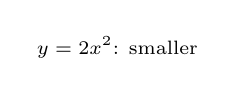
\begin{tikzpicture}[x=.38cm,y=.19cm]
  \roosterleeg{-4}{1}{4}{-2}{2}{10}\xgetallen{-2,2}\ygetallen{2,4,6,8}
  \parabool[tweede,thin]{1}{0}{0}{-3.2}{3.2}
  \parabool{2}{0}{0}{-2.25}{2.25}
  \node[font=\scriptsize] at (0,-4.4) {$y = 2x^2$: smaller};
\end{tikzpicture}\qquad
\begin{tikzpicture}[x=.38cm,y=.19cm]
  \roosterleeg{-4}{1}{4}{-2}{2}{10}\xgetallen{-2,2}\ygetallen{2,4,6,8}
  \parabool[tweede,thin]{1}{0}{0}{-3.2}{3.2}
  \parabool{.5}{0}{0}{-4.2}{4.2}
  \node[font=\scriptsize] at (0,-4.4) {$y = \tfrac12 x^2$: breder};
\end{tikzpicture}\qquad
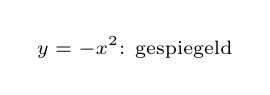
\begin{tikzpicture}[x=.38cm,y=.19cm]
  \roosterleeg{-4}{1}{4}{-10}{2}{10}\xgetallen{-2,2}\ygetallen{-8,-4,4,8}
  \parabool[tweede,thin]{1}{0}{0}{-3.2}{3.2}
  \parabool{-1}{0}{0}{-3.2}{3.2}
  \node[font=\scriptsize] at (0,-12.4) {$y = -x^2$: gespiegeld};
\end{tikzpicture}}

Al deze grafieken zijn parabolen. Ze hebben hun top in de oorsprong en de $y$-as als symmetrieas, maar de top is niet altijd het laagste punt: bij $y = -x^2$ is het het hoogste punt.

\begin{theorie}
De grafiek van $\formule{f(x) = ax^2}$ met $a \neq 0$ is een \textbf{\textcolor{accent}{parabool}}.

De \textbf{\textcolor{accent}{top}} van een parabool is haar laagste of haar hoogste punt. De verticale rechte door de top is de \textbf{\textcolor{accent}{symmetrieas}}.

Voor $y = ax^2$ is de top $\formule{(0, 0)}$ en de symmetrieas de $y$-as, met vergelijking $\formule{x = 0}$.
\end{theorie}

\subsection{Het teken van \texorpdfstring{$a$}{a}}

Waarom ligt $y = -x^2$ onder de $x$-as? Een kwadraat $x^2$ is nooit negatief. Vermenigvuldig je het met een positief getal, dan blijft het positief of nul. Vermenigvuldig je het met een negatief getal, dan wordt het negatief of nul. Het teken van $a$ beslist dus of de parabool naar boven of naar onder openstaat.

\begin{theorie}
\begin{stelling}{Het teken van $a$}
De parabool $y = ax^2$ is

\qquad naar \textbf{\textcolor{accent}{boven geopend}} als $\formule{a > 0}$: de top is het laagste punt;

\qquad naar \textbf{\textcolor{accent}{onder geopend}} als $\formule{a < 0}$: de top is het hoogste punt.
\end{stelling}
\end{theorie}

Een parabool die naar boven openstaat, lijkt op een dal; een parabool die naar onder openstaat, op een berg. De parabolen $y = ax^2$ en $y = -ax^2$ zijn elkaars spiegelbeeld ten opzichte van de $x$-as: elke hoogte krijgt het tegengestelde teken.

\subsection{De grootte van \texorpdfstring{$a$}{a}}

Waarom is $y = 2x^2$ smaller dan $y = x^2$? Bij elke $x$ is de hoogte twee keer zo groot. Bij $x = 1$ is de hoogte precies $a$: zo zie je meteen hoe snel de parabool vanaf de top stijgt of daalt. Hoe groter dat getal (zonder teken), hoe sneller ze stijgt, en hoe smaller ze lijkt.

\begin{theorie}
\begin{stelling}{De grootte van $a$}
Hoe groter $\formule{\abs{a}}$, hoe \textbf{\textcolor{accent}{smaller}} de parabool $y = ax^2$.

Hoe dichter $\abs{a}$ bij $0$ ligt, hoe \textbf{\textcolor{accent}{breder}} de parabool.
\end{stelling}
\end{theorie}

Hier is $\abs{a}$ het getal $a$ zonder teken: $\abs{-3} = 3$. Zo is $y = -3x^2$ smaller dan $y = 2x^2$, ook al is $-3$ kleiner dan $2$. Is $\abs{a} > 1$, dan is de parabool smaller dan $y = x^2$; is $\abs{a} < 1$, dan is ze breder.

\voorbeeld{}{Teken de grafiek van $f(x) = -\tfrac12 x^2$.\label{vb:h1-teken}}{%
\uitleg{Hier is $a = -\tfrac12$: de parabool is naar onder geopend, en breder dan $y = x^2$. We maken een tabel die symmetrisch is rond $0$. Even getallen geven mooie uitkomsten.}
\naast{\waardetabel{7}{-4 & -2 & -1 & 0 & 1 & 2 & 4}{-8 & -2 & -0,5 & 0 & -0,5 & -2 & -8}

\medskip
\textit{Bijvoorbeeld $f(-4) = -\tfrac12 \cdot (-4)^2 = -\tfrac12 \cdot 16 = -8$. Eerst kwadrateren, dan vermenigvuldigen.}

\medskip
\textit{We tekenen de punten en verbinden ze met een vloeiende kromme. De top $(0, 0)$ is het hoogste punt, en de grafiek is symmetrisch ten opzichte van de $y$-as.}}{\begin{tikzpicture}[x=.5cm,y=.36cm]
  \rooster{-4}{1}{4}{-8}{1}{1}
  \parabool{-.5}{0}{0}{-4.1}{4.1}
  \foreach \a in {-4,-2,-1,1,2,4}{\punt{\a}{-\a*\a/2}}
  \toppunt[above right]{0}{0}{top}
\end{tikzpicture}}}

\begin{werkwijze}
Maak een tabel met waarden van $x$ die symmetrisch liggen rond $0$, zoals $-3$ tot $3$. Kwadrateer telkens eerst, en vermenigvuldig dan met $a$. Teken de punten en verbind ze met een vloeiende kromme, met de top in de oorsprong. Controleer: is de parabool naar de goede kant geopend?
\end{werkwijze}

\begin{oefeningen}
\oef{h1-tekenax}
\end{oefeningen}

\subsection{Twee keer zo ver, vier keer zo hoog}

Bij een eerstegraadsfunctie $y = mx$ verdubbelt $y$ als $x$ verdubbelt. Bij $y = ax^2$ is dat anders. Neem $y = 3x^2$: bij $x = 2$ is $y = 12$, bij $x = 4$ is $y = 48$, vier keer zoveel. Dat komt doordat $(2x)^2 = 4x^2$: het getal $2$ wordt ook gekwadrateerd. Wordt $x$ drie keer zo groot, dan wordt $y$ negen keer zo groot.

\voorbeeld{}{Een pizzeria verkoopt ronde pizza's. De hoeveelheid deeg en beleg is evenredig met de oppervlakte, en die is $A = \pi r^2$. De kleine pizza heeft een straal van $12$ cm, de grote van $18$ cm. Hoeveel keer zoveel pizza krijg je bij de grote?\label{vb:h1-pizza}}{%
\uitleg{De oppervlakte is van de vorm $a \cdot r^2$, met $a = \pi$. De straal wordt $\tfrac{18}{12} = 1,5$ keer zo groot.}
\begin{stappen}
\frac{18}{12} = 1,5 & De straal wordt $1,5$ keer zo groot. \\[1ex]
1,5^2 = 2,25 & De oppervlakte wordt $1,5^2$ keer zo groot. \\[1ex]
\frac{\pi \cdot 18^2}{\pi \cdot 12^2} = \frac{324}{144} = 2,25 & Controle met de formule.
\end{stappen}
De grote pizza is $2,25$ keer zo groot, niet $1,5$ keer. Kost ze minder dan $2,25$ keer de prijs van de kleine, dan is ze voordeliger.}

\begin{oefeningen}
\oef{h1-viermaal}
\end{oefeningen}

\subsection{Het voorschrift bij een grafiek}

Je ziet een parabool met de top in de oorsprong. Welk getal $a$ hoort erbij? Elk punt $(x, y)$ van de grafiek voldoet aan $y = ax^2$. Ken je één punt (niet de top), dan vul je het in en reken je $a$ uit.

\voorbeeld{}{Een parabool met top in de oorsprong gaat door het punt $(2, -6)$. Geef het voorschrift.\label{vb:h1-voorschrift}}{%
\uitleg{De top ligt in de oorsprong, dus het voorschrift heeft de vorm $y = ax^2$. We vullen het punt in en lossen op naar $a$.}
\naast{\begin{stappenvrij}{3.5cm}{5.4cm}
-6 = a \cdot 2^2 & Vul $x = 2$ en $y = -6$ in. \\
-6 = 4a & Eerst het kwadraat. \\
a = -\dfrac64 = -1,5 & Deel beide leden door $4$. \\[1ex]
y = -1,5x^2 & Het voorschrift.
\end{stappenvrij}
\textit{Controle: ook het gespiegelde punt $(-2, -6)$ ligt erop, want $-1,5 \cdot (-2)^2 = -6$. En $a < 0$ past bij een parabool die naar onder openstaat.}}{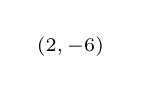
\begin{tikzpicture}[x=.6cm,y=.4cm]
  \rooster{-3}{1}{3}{-7}{1}{1}
  \parabool{-1.5}{0}{0}{-2.15}{2.15}
  \punt{2}{-6}\node[right,font=\scriptsize] at (2,-6) {$(2, -6)$};
\end{tikzpicture}}}

Een snelle controle op een rooster: ga vanaf de top $1$ opzij. Daar is de hoogte $a \cdot 1^2 = a$. Bij $y = -1,5x^2$ ga je dus $1$ opzij en $1,5$ omlaag.

\begin{oefeningen}
\oef{h1-voorschriftax}
\end{oefeningen}

\subsection{Hoe snel stijgt of daalt de parabool?}

Rechts van de top stijgt de parabool $y = x^2$, maar niet overal even snel. In de tabel van sectie 1 zag je het al: bij elke stap van $1$ naar rechts komt er eerst $1$ bij, dan $3$, dan $5$. De stappen omhoog worden steeds groter, en de grafiek wordt steeds steiler. Links van de top is het omgekeerd. Van $x = -3$ naar $x = 0$ daalt $x^2$ eerst met $5$, dan met $3$, dan met $1$: de stappen omlaag worden steeds kleiner, en vlak bij de top is de grafiek bijna vlak.

\figuren{\begin{tikzpicture}[x=.6cm,y=.3cm]
  \rooster{-3}{1}{3}{-1}{1}{9}
  \parabool{1}{0}{0}{-3.1}{3.1}
  \trapje{0}{0}{1}{1}{}{$1$}\trapje{1}{1}{1}{3}{}{$3$}\trapje{2}{4}{1}{5}{}{$5$}
  \foreach \a in {-3,...,3}{\punt{\a}{\a*\a}}
\end{tikzpicture}}

\begin{theorie}
Een functie heeft op een interval een \textbf{\textcolor{accent}{toenemende stijging}} als ze daar stijgt, en steeds steiler: bij gelijke stappen in $x$ worden de stappen omhoog steeds groter. Worden ze steeds kleiner, dan heeft ze een \textbf{\textcolor{accent}{afnemende stijging}}.

\vspace{1mm}
Zo heeft een dalende functie een \textbf{\textcolor{accent}{toenemende daling}} als de stappen omlaag steeds groter worden, en een \textbf{\textcolor{accent}{afnemende daling}} als ze steeds kleiner worden.
\end{theorie}

De functie $f(x) = x^2$ heeft dus een afnemende daling op $\ivog{\minf}{0}$ en een toenemende stijging op $\ivgo{0}{\pinf}$. Bij $y = ax^2$ met $a > 0$ worden alle stappen met $a$ vermenigvuldigd: groter of kleiner, maar het patroon blijft. Bij $a < 0$ keert alles om, want de parabool is gespiegeld. Links van de top stijgt ze dan, steeds minder steil, en rechts daalt ze, steeds steiler. Een rechte stijgt of daalt overal even snel: dat is het grote verschil met een parabool.

\begin{oefeningen}
\oef{h1-verloop}
\end{oefeningen}

\subsection{Kenmerken}

De kenmerken van $f(x) = ax^2$ volgen uit de vorm van de parabool. Het domein is altijd $\R$. De nulwaarde is $0$: dat zie je op de grafiek, want alleen de top ligt op de $x$-as, en ook algebraïsch, want uit $ax^2 = 0$ volgt $x^2 = 0$ (deel door $a \neq 0$), dus $x = 0$. Het snijpunt met de $y$-as is dus de oorsprong. De rest hangt af van het teken van $a$.

\begin{theorie}
{\centering\renewcommand{\arraystretch}{1.5}\begin{tabular}{|c|c|c|}
\hline
 & $\formule{a > 0}$ & $\formule{a < 0}$ \\ \hline
extremum & minimum $0$ in $x = 0$ & maximum $0$ in $x = 0$ \\ \hline
bereik & $\formule{\ivgo{0}{\pinf}}$ & $\formule{\ivog{\minf}{0}}$ \\ \hline
dalend op & $\ivog{\minf}{0}$: afnemende daling & $\ivgo{0}{\pinf}$: toenemende daling \\ \hline
stijgend op & $\ivgo{0}{\pinf}$: toenemende stijging & $\ivog{\minf}{0}$: afnemende stijging \\ \hline
nulwaarde & $0$ & $0$ \\ \hline
tekenschema & \tekenschema{3}{ & 0 & }{+ & 0 & +} & \tekenschema{3}{ & 0 & }{- & 0 & -} \\ \hline
\end{tabular}\par}
\end{theorie}

Je hoeft deze tabel niet van buiten te leren: maak een schets van de parabool, en lees de kenmerken af. Het tekenschema maak je zoals in het handboek Functies: bij $a > 0$ ligt de hele parabool boven de $x$-as, behalve de top.

\voorbeeld{}{Geef de kenmerken van $f(x) = -3x^2$.\label{vb:h1-kenmerken}}{%
\naast{\uitleg{Hier is $a = -3 < 0$: een smalle parabool die naar onder openstaat. We maken een schets en lezen af.}
\begin{stappenvrij}{3.7cm}{5.2cm}
\dom f = \R & Elk getal mag je invullen. \\
\ber f = \ivog{\minf}{0} & De top is het hoogste punt. \\
\text{maximum } 0 \text{ in } x = 0 & De top is $(0, 0)$. \\
\text{stijgend op } \ivog{\minf}{0} & Links van de top gaat het omhoog, steeds minder steil: afnemende stijging. \\
\text{dalend op } \ivgo{0}{\pinf} & Rechts gaat het omlaag, steeds steiler: toenemende daling. \\
\text{nulwaarde } 0 & Alleen de top ligt op de $x$-as. \\
\tekenschema{3}{ & 0 & }{- & 0 & -} & Op de top na ligt de parabool onder de $x$-as.
\end{stappenvrij}}{\begin{tikzpicture}[x=.8cm,y=.4cm]
  \rooster{-2}{1}{2}{-6}{1}{1}
  \parabool[<->,>=stealth]{-3}{0}{0}{-1.45}{1.45}
  \toppunt[above right]{0}{0}{}
\end{tikzpicture}}}

\begin{oefeningen}
\oef{h1-kenmerkenax}
\end{oefeningen}

\begin{alleenvoor}{1}
%========================================================================================
\section{Toepassingen}

\subsection{De vergelijking \texorpdfstring{$ax^2 = k$}{ax² = k}}

In veel problemen ken je de functiewaarde en zoek je $x$. Bij welke $x$ is $3x^2 = 75$? Op de grafiek zoek je de snijpunten van de parabool met de horizontale rechte $y = 75$. Met algebra deel je eerst door $a$, en dan heb je een vergelijking $x^2 = \ldots$ zoals in het handboek Reële getallen.

\voorbeeld{}{Los op: $3x^2 = 75$.\label{vb:h1-vgl}}{%
\naast{\uitleg{We brengen de vergelijking in de vorm $x^2 = \ldots$. De oplossingen zijn de twee vierkantswortels van dat getal: vergeet de negatieve niet.}
\begin{stappenvrij}{3.4cm}{5.4cm}
3x^2 = 75 & \\
x^2 = 25 & Deel beide leden door $3$. \\
x = 5 \ \text{ of } \ x = -5 & Twee getallen hebben $25$ als kwadraat.
\end{stappenvrij}
\textit{Controle: $3 \cdot (-5)^2 = 3 \cdot 25 = 75$. Op de grafiek snijdt de rechte $y = 75$ de parabool $y = 3x^2$ in twee punten, symmetrisch ten opzichte van de $y$-as.}}{\begin{tikzpicture}[x=.36cm,y=.022cm]
  \roosterleeg{-6}{1}{6}{0}{25}{100}
  \xgetallen{-5,5}\ygetallen{25,50,75}
  \parabool{3}{0}{0}{-5.7}{5.7}
  \draw[hulplijn] (-6,75) -- (6,75);
  \aflezen{5}{75}\aflezen{-5}{75}
  \punt{5}{75}\punt{-5}{75}
\end{tikzpicture}}}

Niet elke vergelijking van deze vorm heeft twee oplossingen. Ligt de rechte $y = k$ aan de andere kant van de $x$-as dan de parabool, dan snijden ze elkaar niet.

\voorbeeld{}{Los op: $-2x^2 = 8$.\label{vb:h1-geen}}{%
\naast{\uitleg{We delen door $-2$. Het teken verandert, want we delen door een negatief getal.}
\begin{stappenvrij}{3.4cm}{5.4cm}
-2x^2 = 8 & \\
x^2 = -4 & Deel beide leden door $-2$. \\
\text{geen oplossing} & Een kwadraat is nooit negatief.
\end{stappenvrij}
\textit{Op de grafiek: de parabool $y = -2x^2$ ligt volledig op of onder de $x$-as, de rechte $y = 8$ erboven.}}{\begin{tikzpicture}[x=.4cm,y=.2cm]
  \roosterleeg{-3}{1}{3}{-10}{2}{10}
  \xgetallen{-2,2}\ygetallen{-8,-4,4,8}
  \parabool{-2}{0}{0}{-2.2}{2.2}
  \draw[hulplijn] (-3,8) -- (3,8);
\end{tikzpicture}}}

\begin{werkwijze}
Deel beide leden door $a$, zodat je $x^2 = \tfrac ka$ krijgt. Is dat getal positief, dan zijn er twee oplossingen: $x = \sqrt{\tfrac ka}$ en $x = -\sqrt{\tfrac ka}$. Is het $0$, dan is $x = 0$ de enige oplossing. Is het negatief, dan is er geen oplossing. In een context houd je alleen de oplossingen over die zin hebben.
\end{werkwijze}

\begin{oefeningen}
\oef{h1-vglax}
\end{oefeningen}

\subsection{Problemen met een kwadratisch verband}

Een verband van de vorm $y = ax^2$ heet \textit{kwadratisch}. In een context betekenen $x$ en $y$ iets, en vaak heeft alleen een deel van de grafiek zin: een tijd of een snelheid is niet negatief.

\voorbeeld{}{Een steen valt van een brug. Na $t$ seconden is hij ongeveer $s = 5t^2$ meter gevallen. Hoe ver is de steen na $2$ seconden gevallen? En na hoeveel seconden raakt hij het water, $45$ m lager?\label{vb:h1-val}}{%
\naast{\uitleg{De eerste vraag is een functiewaarde. Bij de tweede vraag ken je $s$ en zoek je $t$: dat is een vergelijking.}
\begin{stappenvrij}{3.6cm}{5cm}
s = 5 \cdot 2^2 = 20 & Na $2$ s is hij $20$ m gevallen. \\[1ex]
5t^2 = 45 & Wanneer is $s = 45$? \\
t^2 = 9 & Deel beide leden door $5$. \\
t = 3 & $t = -3$ heeft hier geen zin.
\end{stappenvrij}
\textit{De steen raakt na $3$ s het water. In de eerste seconde valt hij $5$ m, in de derde seconde al $45 - 20 = 25$ m: hij valt steeds sneller.}}{\begin{tikzpicture}[x=.8cm,y=.04cm]
  \roosterleeg[$t$ (s)][$s$ (m)]{0}{1}{3.5}{0}{10}{50}
  \xgetallen{1,2,3}\ygetallen{10,20,30,40,50}\oorsprong
  \parabool{5}{0}{0}{0}{3.15}
  \draw[hulplijn] (0,45) -- (3.5,45);
  \aflezen{2}{20}\aflezen{3}{45}\punt{2}{20}\punt{3}{45}
\end{tikzpicture}}}

\begin{oefeningen}
\oef{h1-context}
\end{oefeningen}

\subsection{De boog van de brug}

Nu kunnen we het probleem van de brug oplossen. Het belangrijkste idee: \textit{jij} kiest waar je de assen tekent. Leg je de oorsprong in de top van de boog, dan is de boog een parabool met top in de oorsprong, met een voorschrift $y = ax^2$.

\voorbeeld{}{Terug naar het probleem. De boog is $40$ m breed en $10$ m hoog. Hoe hoog is de boog op $5$ m van een voet? Hoe breed is de strook waar een boot van $8$ m hoog onder de boog door kan?\label{vb:h1-terug}}{%
\uitleg{We leggen de oorsprong in de top. De voeten liggen dan $20$ m links en rechts van de top en $10$ m lager: in $(-20, -10)$ en $(20, -10)$. Het water ligt op hoogte $y = -10$.}
\naast{\begin{stappenvrij}{3.5cm}{4.5cm}
-10 = a \cdot 20^2 & De voet $(20, -10)$ ligt op de boog. \\
a = -\dfrac{10}{400} = -\dfrac1{40} & Deel door $400$. \\[1ex]
y = -\dfrac{1}{40}x^2 & Het voorschrift van de boog. \\[1ex]
y = -\dfrac{15^2}{40} = -5,625 & $5$ m van de voet is $x = 15$. \\[1ex]
-5,625 + 10 = 4,375 & De hoogte boven het water.
\end{stappenvrij}}{\begin{tikzpicture}[x=.09cm,y=.18cm]
  \fill[accent!10] (-22,-11.5) rectangle (22,-10);
  \roosterleeg{-22}{2}{22}{-11.5}{2}{1}
  \xgetallen{-20,-10,10,20}\ygetallen{-10,-5}
  \draw[grijs] (-22,-10) -- (22,-10);
  \parabool{-.025}{0}{0}{-20}{20}
  \punt{20}{-10}\punt{-20}{-10}
  \draw[hulplijn] (-22,-2) -- (22,-2);
  \punt{8.94}{-2}\punt{-8.94}{-2}
  \draw[inkt,thick] (15,-10) -- (15,-5.625);\punt[inkt]{15}{-5.625}
\end{tikzpicture}}
\begin{stappen}
-2 = -\dfrac{1}{40}x^2 & De kajuit van $8$ m komt tot $2$ m onder de top: $y = -2$. \\[1ex]
x^2 = 80 & Beide leden maal $-40$. \\
x = \pm\sqrt{80} \approx \pm 8,94 & Van $-8,94$ tot $8,94$ is de boog hoger dan $8$ m.
\end{stappen}
Op $5$ m van een voet is de boog $4,375$ m hoog, ongeveer $4,4$ m. Een boot van $8$ m hoog kan door een strook van $2 \cdot 8,94 \approx 17,9$ m breed, in het midden van de rivier.}
\end{alleenvoor}

\begin{alleenvoor}{2,3,4,5}
%========================================================================================
\section{De parabool verschuiven}

De top van een parabool ligt niet altijd in de oorsprong. Bij de brug kun je de oorsprong bijvoorbeeld op het water leggen, bij een voet van de boog. Dan ligt de top in $(20, 10)$. Welk voorschrift hoort dan bij de boog? We onderzoeken eerst wat er gebeurt als je de parabool verticaal en horizontaal verschuift.

\subsection{Verticaal verschuiven}

Vergelijk $y = x^2$ met $y = x^2 + 3$ en $y = x^2 - 2$. Bij elke $x$ tel je bij het kwadraat $3$ op, of trek je er $2$ van af.

\naast{\waardetabel[$x$][$y$]{5}{-2 & -1 & 0 & 1 & 2}{4 & 1 & 0 & 1 & 4}

\smallskip
\waardetabel[$x$][$y + 3$]{5}{-2 & -1 & 0 & 1 & 2}{7 & 4 & 3 & 4 & 7}

\medskip
Elk punt van $y = x^2$ gaat $3$ eenheden omhoog. De vorm blijft dezelfde, alleen de plaats verandert. De top gaat van $(0, 0)$ naar $(0, 3)$. Bij $y = x^2 - 2$ gaat alles $2$ eenheden omlaag, naar de top $(0, -2)$.}{\begin{tikzpicture}[x=.55cm,y=.3cm]
  \rooster{-3}{1}{3}{-3}{1}{9}
  \parabool[tweede,thin]{1}{0}{0}{-3}{3}
  \parabool{1}{0}{3}{-2.45}{2.45}
  \parabool[inkt,thick]{1}{0}{-2}{-3}{3}
  \foreach \a in {-2,-1,1,2}{\draw[grijs,->,>=stealth] (\a,\a*\a) -- (\a,\a*\a+2.8);}
  \node[accent,font=\scriptsize,right] at (2.4,8.5) {$y = x^2 + 3$};
  \node[inkt,font=\scriptsize,right] at (3,6.5) {$y = x^2 - 2$};
\end{tikzpicture}}

\begin{theorie}
\begin{stelling}{Verticaal verschuiven}
De grafiek van $\formule{y = ax^2 + q}$ is de parabool $y = ax^2$, verticaal verschoven over $q$: naar boven als $q > 0$, naar onder als $q < 0$.

De top is $\formule{(0, q)}$.
\end{stelling}
\end{theorie}

\subsection{Horizontaal verschuiven}

Nu de functie $y = (x - 3)^2$. Waar ligt haar top? Het kwadraat is het kleinst, namelijk $0$, als $x - 3 = 0$, dus bij $x = 3$. In de tabel zie je dezelfde getallen als bij $y = x^2$, maar ze staan $3$ plaatsen verder naar rechts.

\naast{\waardetabel[$x$][$x^2$]{7}{-3 & -2 & -1 & 0 & 1 & 2 & 3}{9 & 4 & 1 & 0 & 1 & 4 & 9}

\smallskip
\waardetabel[$x$][$(x - 3)^2$]{7}{0 & 1 & 2 & 3 & 4 & 5 & 6}{9 & 4 & 1 & 0 & 1 & 4 & 9}

\medskip
De parabool $y = (x - 3)^2$ is dus $y = x^2$, $3$ eenheden naar \textit{rechts} verschoven. Dat voelt misschien vreemd: er staat een minteken, en toch gaat het naar rechts. Maar wat $y = x^2$ bij $x = 0$ doet, doet $y = (x - 3)^2$ pas bij $x = 3$. Zo is $y = (x + 2)^2$ verschoven naar links, met de top bij $x = -2$.}{\begin{tikzpicture}[x=.45cm,y=.3cm]
  \rooster{-3}{1}{6}{-1}{1}{9}
  \parabool[tweede,thin]{1}{0}{0}{-3}{3}
  \parabool{1}{3}{0}{0}{6}
  \draw[grijs,->,>=stealth] (-2,4) -- (0.8,4);
  \draw[grijs,->,>=stealth] (2,4) -- (4.8,4);
  \node[accent,font=\scriptsize,right] at (5.2,8) {$(x - 3)^2$};
\end{tikzpicture}}

\begin{theorie}
\begin{stelling}{Horizontaal verschuiven}
De grafiek van $\formule{y = a(x - p)^2}$ is de parabool $y = ax^2$, horizontaal verschoven over $p$: naar rechts als $p > 0$, naar links als $p < 0$.

De top is $\formule{(p, 0)}$ en de symmetrieas is de rechte $\formule{x = p}$.
\end{stelling}
\end{theorie}

Let op het teken. Bij $y = 2(x + 4)^2$ schrijf je eerst $x + 4 = x - (-4)$: dan is $p = -4$, de top is $(-4, 0)$ en de parabool is $4$ eenheden naar links verschoven.

\begin{oefeningen}
\oef{h1-verschuif}
\end{oefeningen}

\subsection{De topvorm}

Je kunt beide verschuivingen combineren. Neem de parabool $y = ax^2$, verschuif ze $p$ naar rechts en dan $q$ naar boven. Dan krijg je $y = a(x - p)^2 + q$. De top gaat mee: van $(0, 0)$ naar $(p, q)$. De vorm blijft die van $y = ax^2$.

\begin{theorie}
Het voorschrift $\formule{y = a(x - p)^2 + q}$ met $a \neq 0$ heet de \textbf{\textcolor{accent}{topvorm}} van een parabool.

\begin{stelling}{Top en symmetrieas}
De parabool $y = a(x - p)^2 + q$ heeft als top $\formule{(p, q)}$ en als symmetrieas de rechte $\formule{x = p}$. Ze heeft dezelfde vorm als $y = ax^2$.
\end{stelling}
\alleenvoor{5}{\begin{bewijs}
Neem twee punten die even ver links en rechts van $x = p$ liggen: $x = p + h$ en $x = p - h$. Dan is
\bewijsregel{a\bigl((p + h) - p\bigr)^2 + q = ah^2 + q \quad\text{en}\quad a\bigl((p - h) - p\bigr)^2 + q = a(-h)^2 + q = ah^2 + q.}
Beide punten liggen op dezelfde hoogte, dus de rechte $x = p$ is een symmetrieas. Omdat $h^2 \geqslant 0$, ligt $ah^2 + q$ voor $a > 0$ nooit onder $q$ en voor $a < 0$ nooit boven $q$: het punt $(p, q)$ is het laagste of het hoogste punt.
\end{bewijs}}
\end{theorie}

\alleenvoor{2,3,4}{Waarom is $x = p$ de symmetrieas? Ga je vanaf $x = p$ een afstand $h$ naar rechts of naar links, dan is $x - p$ gelijk aan $h$ of aan $-h$. Het kwadraat is in beide gevallen $h^2$, dus je komt op dezelfde hoogte uit. }Het getal $a$ zegt zoals vroeger of de parabool naar boven of naar onder openstaat, en hoe breed ze is.

\voorbeeld{}{Teken de grafiek van $y = 2(x + 1)^2 - 3$.\label{vb:h1-topvorm}}{%
\uitleg{We lezen de top af en tekenen vanuit de top de vorm van $y = 2x^2$: $1$ opzij is $2 \cdot 1^2 = 2$ omhoog, $2$ opzij is $2 \cdot 2^2 = 8$ omhoog.}
\naast{\begin{stappenvrij}{3.9cm}{4.6cm}
y = 2\bigl(x - (-1)\bigr)^2 + (-3) & Schrijf in de topvorm: $p = -1$, $q = -3$. \\
\text{top } (-1, -3) & Symmetrieas $x = -1$. \\
a = 2 > 0 & Naar boven geopend, smaller dan $y = x^2$. \\
(0, -1) \text{ en } (-2, -1) & $1$ opzij, $2$ omhoog. \\
(1, 5) \text{ en } (-3, 5) & $2$ opzij, $8$ omhoog.
\end{stappenvrij}
\textit{Controle met het voorschrift: bij $x = 1$ is $y = 2 \cdot 2^2 - 3 = 5$.}}{\begin{tikzpicture}[x=.6cm,y=.33cm]
  \rooster{-4}{1}{2}{-4}{1}{6}
  \symas{-1}{-4}{6.3}
  \parabool{2}{-1}{-3}{-3.2}{1.2}
  \toppunt[below right]{-1}{-3}{$(-1, -3)$}
  \punt{0}{-1}\punt{-2}{-1}\punt{1}{5}\punt{-3}{5}
  \trapje{-1}{-3}{1}{2}{$1$}{$2$}
\end{tikzpicture}}}

\begin{werkwijze}
Schrijf het voorschrift in de vorm $y = a(x - p)^2 + q$ en lees de top $(p, q)$ af. Teken de top en de symmetrieas $x = p$. Ga vanaf de top $1$ opzij en $a$ omhoog (of omlaag als $a < 0$), $2$ opzij en $4a$, $3$ opzij en $9a$. Spiegel die punten om de as, en verbind alles met een vloeiende kromme.
\end{werkwijze}

\begin{oefeningen}
\oef{h1-tekentop}
\end{oefeningen}

%========================================================================================
\section{Het voorschrift aflezen}

Nu omgekeerd: je ziet een parabool, en je zoekt het voorschrift. In de topvorm $y = a(x - p)^2 + q$ staan drie getallen. De top geeft er al twee: $p$ en $q$. Voor het derde getal, $a$, heb je nog één punt nodig.

\voorbeeld{}{Geef het voorschrift van de parabool hiernaast.\label{vb:h1-aflezen}}{%
\naast{\uitleg{We lezen de top af en kiezen nog een punt van de grafiek dat op een knooppunt van het rooster ligt.}
\begin{stappenvrij}{3.6cm}{5.2cm}
\text{top } (-1, 3) & Dus $p = -1$ en $q = 3$. \\
y = a(x + 1)^2 + 3 & Het voorschrift, met $a$ nog onbekend. \\
-5 = a(1 + 1)^2 + 3 & Het punt $(1, -5)$ ligt op de parabool. \\
-8 = 4a & Trek $3$ af van beide leden. \\
a = -2 & Deel door $4$. \\[1ex]
y = -2(x + 1)^2 + 3 & Het voorschrift.
\end{stappenvrij}
\textit{Controle op het rooster: vanaf de top $1$ opzij gaat de grafiek $2$ omlaag, en dat is $a = -2$.}}{\begin{tikzpicture}[x=.6cm,y=.33cm]
  \rooster{-4}{1}{2}{-6}{1}{4}
  \parabool{-2}{-1}{3}{-3.15}{1.15}
  \toppunt[above]{-1}{3}{}
  \punt{1}{-5}\punt{0}{1}
\end{tikzpicture}}}

\begin{werkwijze}
Lees de top $(p, q)$ af en vul in: $y = a(x - p)^2 + q$. Kies een ander punt van de grafiek, liefst op een knooppunt van het rooster, en vul zijn coördinaten in. Los de vergelijking op naar $a$. Controleer: $1$ opzij vanaf de top moet je $a$ omhoog of omlaag gaan.
\end{werkwijze}

\begin{oefeningen}
\oef{h1-aflezen}
\end{oefeningen}

Dezelfde aanpak werkt zonder tekening: ken je de top en één ander punt, dan ken je de parabool.

\voorbeeld{}{Terug naar het probleem. De boog is $40$ m breed en $10$ m hoog. Hoe hoog is de boog op $5$ m van een voet? Hoe breed is de strook waar een boot van $8$ m hoog onder de boog door kan?\label{vb:h1-terug}}{%
\uitleg{We leggen de oorsprong op het water, bij de linkervoet. Dan ligt de top in $(20, 10)$ en de andere voet in $(40, 0)$. De oorsprong zelf ligt ook op de boog.}
\naast{\begin{stappenvrij}{4.6cm}{3.6cm}
y = a(x - 20)^2 + 10 & De top is $(20, 10)$. \\
0 = a(0 - 20)^2 + 10 & De voet $(0, 0)$ ligt op de boog. \\
a = -\dfrac{10}{400} = -\dfrac{1}{40} & $400a = -10$. \\[1ex]
y = -\dfrac{1}{40}(x - 20)^2 + 10 & Het voorschrift van de boog. \\[1ex]
y(5) = -\dfrac{15^2}{40} + 10 = 4,375 & De hoogte bij $x = 5$.
\end{stappenvrij}}{\begin{tikzpicture}[x=.08cm,y=.16cm]
  \fill[accent!10] (-2,-1.5) rectangle (42,0);
  \roosterleeg{-2}{2}{42}{-1.5}{2}{11}
  \xgetallen{10,20,30,40}\ygetallen{5,10}
  \parabool{-.025}{20}{10}{0}{40}
  \toppunt[above]{20}{10}{}
  \punt{0}{0}\punt{40}{0}
  \draw[hulplijn] (-2,8) -- (42,8);
  \punt{11.06}{8}\punt{28.94}{8}
  \draw[inkt,thick] (5,0) -- (5,4.375);\punt[inkt]{5}{4.375}
\end{tikzpicture}}
\begin{stappen}
-\dfrac{1}{40}(x - 20)^2 + 10 = 8 & Waar is de boog $8$ m hoog? \\[1ex]
(x - 20)^2 = 80 & Trek $10$ af en vermenigvuldig met $-40$. \\
x - 20 = \pm\sqrt{80} \approx \pm 8,94 & Twee getallen hebben $80$ als kwadraat. \\
x \approx 11,06 \ \text{ of } \ x \approx 28,94 & De strook loopt van $11,06$ m tot $28,94$ m.
\end{stappen}
Op $5$ m van een voet is de boog $4,375$ m hoog, ongeveer $4,4$ m. Een boot van $8$ m hoog kan door een strook van $28,94 - 11,06 \approx 17,9$ m breed. Met de oorsprong in de top was het voorschrift eenvoudiger geweest: $y = -\tfrac{1}{40}x^2$. De keuze van de assen verandert het voorschrift, maar niet het antwoord.}

\subsection{Twee punten op dezelfde hoogte}

Bij de brug lagen de twee voeten op dezelfde hoogte, en de top lag er precies tussen. Dat is geen toeval. De symmetrieas is een spiegel: een punt links van de as heeft rechts een spiegelbeeld op dezelfde hoogte, even ver van de as. Omgekeerd: ken je twee punten van een parabool op dezelfde hoogte, dan ligt de as precies in het midden, ook als je de top niet kent.

\begin{theorie}
\begin{stelling}{Twee punten op dezelfde hoogte}
Liggen twee verschillende punten $(x_1, y)$ en $(x_2, y)$ op de parabool $y = a(x - p)^2 + q$, dan is

\qquad $\formule{p = \dfrac{x_1 + x_2}{2}}$.

De symmetrieas ligt midden tussen beide punten.
\end{stelling}
\alleenvoor{5}{\begin{bewijs}
Beide punten liggen op de parabool, dus
\bewijsregel{a(x_1 - p)^2 + q = y = a(x_2 - p)^2 + q \iff (x_1 - p)^2 = (x_2 - p)^2,}
na $q$ aftrekken en delen door $a \neq 0$. Twee getallen met hetzelfde kwadraat zijn gelijk of tegengesteld. Gelijk kan niet, want dan is $x_1 = x_2$. Dus
\bewijsregel{x_1 - p = -(x_2 - p) \iff x_1 + x_2 = 2p \iff p = \frac{x_1 + x_2}{2}.}
\end{bewijs}}
\end{theorie}

\alleenvoor{2,3,4}{Waarom klopt dat? Op dezelfde hoogte is $a(x_1 - p)^2 + q = a(x_2 - p)^2 + q$, dus $(x_1 - p)^2 = (x_2 - p)^2$. Twee verschillende getallen met hetzelfde kwadraat zijn tegengesteld: $x_1$ ligt even ver links van $p$ als $x_2$ rechts ervan. }Een bijzonder geval zijn de nulwaarden: twee punten op hoogte $0$. De symmetrieas ligt dus midden tussen de nulwaarden. Snijdt een parabool de $x$-as in $-1$ en $5$, dan is haar as $x = \tfrac{-1 + 5}{2} = 2$.

\subsection{Het voorschrift zonder top}

Ken je de top niet, dan heb je drie punten nodig. Liggen er twee op dezelfde hoogte, dan geven ze $p$. Dan blijven er in $y = a(x - p)^2 + q$ nog twee onbekenden over, $a$ en $q$, en daarvoor heb je twee andere punten nodig. Je krijgt twee vergelijkingen. Trek je ze van elkaar af, dan valt $q$ weg.

\voorbeeld{}{Een parabool gaat door de punten $(-1, 5)$, $(3, 5)$ en $(2, -1)$. Geef het voorschrift.\label{vb:h1-zondertop}}{%
\naast{\uitleg{De punten $(-1, 5)$ en $(3, 5)$ liggen op dezelfde hoogte: zij geven de symmetrieas. Voor $a$ en $q$ gebruiken we de twee andere punten.}
\begin{stappenvrij}{3.7cm}{5.1cm}
p = \dfrac{-1 + 3}{2} = 1 & De as ligt in het midden. \\[1ex]
y = a(x - 1)^2 + q & Nog twee onbekenden. \\
5 = 4a + q & Het punt $(3, 5)$. \\
-1 = a + q & Het punt $(2, -1)$. \\
6 = 3a & Trek de vergelijkingen af: $q$ valt weg. \\
a = 2,\ q = -3 & Uit $-1 = 2 + q$. \\[1ex]
y = 2(x - 1)^2 - 3 & Het voorschrift.
\end{stappenvrij}
\textit{Controle met het derde punt: $2 \cdot (-2)^2 - 3 = 5$, dus $(-1, 5)$ ligt erop.}}{\begin{tikzpicture}[x=.55cm,y=.3cm]
  \roosterleeg{-2}{1}{4}{-4}{1}{6}\xgetallen{-1,1,2,3}\ygetallen{-3,-1,5}
  \symas{1}{-4}{6}
  \draw[hulplijn] (-2,5) -- (4,5);
  \parabool{2}{1}{-3}{-1.1}{3.1}
  \toppunt[below right]{1}{-3}{}
  \punt{-1}{5}\punt{3}{5}\punt{2}{-1}
\end{tikzpicture}}}

Ook het snijpunt met de $y$-as en de nulwaarden zijn punten die je kunt gebruiken. Zijn de nulwaarden gegeven, dan geven zij de as.

\voorbeeld{}{Een parabool snijdt de $x$-as in $-1$ en $5$, en de $y$-as in $(0, -5)$. Geef het voorschrift.\label{vb:h1-ysnij}}{%
\naast{\uitleg{De nulwaarden zijn twee punten op hoogte $0$: ze geven de as. Daarna vullen we een nulwaarde en het snijpunt met de $y$-as in.}
\begin{stappenvrij}{3.7cm}{5.1cm}
p = \dfrac{-1 + 5}{2} = 2 & Midden tussen de nulwaarden. \\[1ex]
y = a(x - 2)^2 + q & \\
0 = 9a + q & Het punt $(5, 0)$. \\
-5 = 4a + q & Het punt $(0, -5)$. \\
5 = 5a & Trek af: $a = 1$, $q = -9$. \\[1ex]
y = (x - 2)^2 - 9 & Het voorschrift.
\end{stappenvrij}
\textit{Controle: $(-1 - 2)^2 - 9 = 0$. Het spiegelbeeld van $(0, -5)$ is $(4, -5)$.}}{\begin{tikzpicture}[x=.45cm,y=.22cm]
  \roosterleeg{-2}{1}{6}{-10}{1}{3}\xgetallen{-1,2,4,5}\ygetallen{-9,-5}
  \symas{2}{-10}{3}
  \parabool{1}{2}{-9}{-1.45}{5.45}
  \toppunt[below right]{2}{-9}{}
  \punt{-1}{0}\punt{5}{0}\punt{0}{-5}\punt[inkt]{4}{-5}
\end{tikzpicture}}}

\begin{werkwijze}
Zoek twee punten op dezelfde hoogte (bijvoorbeeld de nulwaarden): $p$ ligt in het midden. Vul $p$ in: $y = a(x - p)^2 + q$. Vul twee andere punten in, zodat je twee vergelijkingen in $a$ en $q$ krijgt. Trek ze van elkaar af: $q$ valt weg en je vindt $a$, daarna $q$. Controleer met het derde punt.
\end{werkwijze}

\begin{oefeningen}
\oef{h1-zondertop}
\end{oefeningen}
\end{alleenvoor}

%========================================================================================
\opdrachtenkop

\begin{oefeningen}
\needspace{6\baselineskip}
\oef{h1-o1}

\needspace{6\baselineskip}
\oef{h1-o2}

\needspace{6\baselineskip}
\oef{h1-o20}

\needspace{6\baselineskip}
\oef{h1-o40}

\needspace{6\baselineskip}
\oef{h1-o3}

\needspace{6\baselineskip}
\oef{h1-o21}

\needspace{6\baselineskip}
\oef{h1-o41}

\needspace{6\baselineskip}
\oef{h1-o4}

\needspace{6\baselineskip}
\oef{h1-o22}

\needspace{6\baselineskip}
\oef{h1-o42}

\needspace{6\baselineskip}
\oef{h1-o5}

\needspace{6\baselineskip}
\oef{h1-o43}

\needspace{6\baselineskip}
\oef{h1-o6}

\needspace{6\baselineskip}
\oef{h1-o7}

\needspace{6\baselineskip}
\oef{h1-o23}

\needspace{6\baselineskip}
\oef{h1-o44}

\needspace{6\baselineskip}
\oef{h1-o8}

\needspace{6\baselineskip}
\oef{h1-o24}

\needspace{6\baselineskip}
\oef{h1-o45}

\needspace{6\baselineskip}
\oef{h1-o9}

\needspace{6\baselineskip}
\oef{h1-o25}

\needspace{6\baselineskip}
\oef{h1-o46}

\needspace{6\baselineskip}
\oef{h1-o10}

\needspace{6\baselineskip}
\oef{h1-o26}

\needspace{6\baselineskip}
\oef{h1-o47}

\needspace{6\baselineskip}
\oef{h1-o11}

\needspace{6\baselineskip}
\oef{h1-o27}

\needspace{6\baselineskip}
\oef{h1-o30}

\needspace{6\baselineskip}
\oef{h1-o12}

\needspace{6\baselineskip}
\oef{h1-o28}

\needspace{6\baselineskip}
\oef{h1-o48}

\needspace{6\baselineskip}
\oef{h1-o13}

\needspace{6\baselineskip}
\oef{h1-o29}

\needspace{6\baselineskip}
\oef{h1-o49}

\needspace{6\baselineskip}
\oef{h1-o51}

\needspace{6\baselineskip}
\oef{h1-o52}
\end{oefeningen}

%----------------------------------------------------------------------------------------
\needspace{14\baselineskip}
\opdrachtsectie{Test jezelf}

\begin{oefeningen}
\needspace{6\baselineskip}
\oef{h1-t1}

\needspace{6\baselineskip}
\oef{h1-t2}

\needspace{6\baselineskip}
\oef{h1-t3}

\needspace{6\baselineskip}
\oef{h1-t4}

\needspace{6\baselineskip}
\oef{h1-t5}

\needspace{6\baselineskip}
\oef{h1-t6}

\needspace{6\baselineskip}
\oef{h1-t7}
\end{oefeningen}

\herhaalschema{%
  \fv{oef:h1-t1}{vb:h1-teken}{oef:h1-o3}%
  \fv{oef:h1-t2}{vb:h1-teken}{oef:h1-tekenax}%
  \fv{oef:h1-t3}{vb:h1-voorschrift}{oef:h1-voorschriftax}%
  \fv{oef:h1-t4}{vb:h1-kenmerken}{oef:h1-kenmerkenax}%
  \alleenvoor{1}{\fv{oef:h1-t5}{vb:h1-vgl}{oef:h1-vglax}}\alleenvoor{2,3,4,5}{\fv{oef:h1-t5}{vb:h1-topvorm}{oef:h1-verschuif}}%
  \alleenvoor{1}{\fv{oef:h1-t6}{vb:h1-val}{oef:h1-context}}\alleenvoor{2,3,4,5}{\fv{oef:h1-t6}{vb:h1-topvorm}{oef:h1-tekentop}}%
  \alleenvoor{1}{\fv{oef:h1-t7}{vb:h1-terug}{oef:h1-o24}}\alleenvoor{2,3,4,5}{\fv{oef:h1-t7}{vb:h1-aflezen}{oef:h1-aflezen}}}

\ifzelfstudie
\section*{Maak je eigen samenvatting}
Sluit dit boek en schrijf in je schrift: hoe de parabool $y = x^2$ eruitziet en waarom ze symmetrisch is, wat een top en een symmetrieas zijn, wat het teken en de grootte van $a$ met de parabool $y = ax^2$ doen, hoe je $a$ vindt uit één punt\alleenvoor{1}{, en hoe je een vergelijking $ax^2 = k$ oplost}\alleenvoor{2,3,4,5}{, wat $p$ en $q$ in de topvorm $y = a(x - p)^2 + q$ doen, hoe je vanuit de top tekent, en hoe je het voorschrift afleest bij een grafiek}. Vergelijk daarna met de kaders.
\fi
